\documentclass{article}
\usepackage{alphalph}
\usepackage{amsmath}
\usepackage{amssymb}
\usepackage{arydshln}
\usepackage{booktabs}
\usepackage{changepage}
\usepackage{csquotes}
\usepackage{enumitem}
\usepackage[margin=2cm]{geometry}
\usepackage{multicol}
\usepackage{rotating}

\usepackage[backend=biber,style=alphabetic]{biblatex}
\addbibresource{\jobname.bib}

\usepackage{acronym}

\usepackage{caption}
\captionsetup{font=small,labelfont=bf,labelsep=period}

\makeatletter
\def\enumalphalphcnt#1{\expandafter\@enumalphalphcnt\csname c@#1\endcsname}
\def\@enumalphalphcnt#1{\alphalph{#1}}
\makeatother
\AddEnumerateCounter{\enumalphalphcnt}{\@enumalphalphcnt}{aa}

\title{Reconstructing the Phylogeny of the Caminalcules \\
       \Large\textsc{biosci \oldstylenums{210} lab report}}
\author{Arman Bilge}
\date{August 28, 2014}

\frenchspacing
\begin{document}

    \maketitle

    \section*{Introduction}

        Phylogenetic trees are powerful tools to learn about evolutionary
            processes.
        A phylogenetic tree is a representation of the speciation events that
            created a group of organisms.
        Specifically, we can learn about the evolution of traits within a group of organisms and identify traits as \emph{symplesiomorphies} (ancestral states), \emph{synampomorphies} (shared derived states), or \emph{autapomorphies} (unique derived states).
        Here, we attempt to reconstruct the phylogeny of the Caminalcules using
            morphological characters due to a lack of DNA data.
        Specifically, we look at two clades, an ingroup clade A (species 1--22) and an outgroup clade B (species 23--29).

    \section*{Data and Phylogenetic Analysis}

        \subsection*{Characters considered}

            I identified some 36 characters to use for reconstrucint the phylogeny of the Calminacules, as described below.
            Characters were chosen on primarily two criteria: their immediate apparentness and their affinity to be summarised concisely and discretely.
            The data matrix (table~1) was assembled by scrutinising each species for its state in each character.

            \begin{multicols}{2}
                \begin{enumerate}[label=\textbf{\enumalphalphcnt*.}]
                    \item Has eyes
                    \item Has appendages at front
                    \item Has distinct head
                    \item Appendages are stubs
                    \item Appendages are tentacles
                    \item Appendages are arms with hands
                    \item Body in distinct sections
                    \item Appendages are wing-like
                    \item Has single or fused eye
                    \item Arms are jointed
                    \item Has one rear appendage
                    \item Has two rear appendages
                    \item Rear appendage is feet
                    \item Hands have nails
                    \item Eyes are on antennae on opposite sides of the head
                    \item Rear appendage is fused to body
                    \item Rear appendage is tail-fin
                    \item Tentacles have sparse spots
                    \item Tentacles have dense spots
                    \item Spots on body are in \enquote{U} pattern
                    \item Head splits into protruding appendages
                    \item Body is bean-shaped
                    \item Spots on body are in row-like pattern
                    \item Tentacles are at least twice as long as neck and head
                    \item Body is covered in patches, spots, and/or dots
                    \item Spots on body are in 4-2-2 pattern
                    \item Head has no eyes and is bluntly shaped
                    \item Tentacles are darkly-coloured
                    \item Wings are rounded
                    \item Middle body section has two thick spots
                    \item Round section of body is large
                    \item Round section of body is small
                    \item Stubs are long
                    \item Stubs are short
                    \item \enquote{M}-pattern on body is readily apparent
                    \item Round wing is small
                \end{enumerate}
            \end{multicols}

            \begin{sidewaystable}
                \centering
                \caption{Data matrix representing how each species was coded for
                             the characters.
                         The dashed-line separates the outgroup species 23--29
                             from the ingroup.
                         Letters refer to characters as described in-text.
                         A value of 1 indicates that the species was positive
                             for that character; 0~indicates negative or not
                             applicable.
                }
                \small
                \begin{tabular}%
                          {r | rrr rrr rrr rrr rrr rrr rrr rrr rrr rrr rrr rrr}
                    \toprule
                    & \multicolumn{36}{c}{\textsc{Character}} \\
                    \textsc{Species}
                        & \textbf{a}
                        & \textbf{b}
                        & \textbf{c}
                        & \textbf{d}
                        & \textbf{e}
                        & \textbf{f}
                        & \textbf{g}
                        & \textbf{h}
                        & \textbf{i}
                        & \textbf{j}
                        & \textbf{k}
                        & \textbf{l}
                        & \textbf{m}
                        & \textbf{n}
                        & \textbf{o}
                        & \textbf{p}
                        & \textbf{q}
                        & \textbf{r}
                        & \textbf{s}
                        & \textbf{t}
                        & \textbf{u}
                        & \textbf{v}
                        & \textbf{w}
                        & \textbf{x}
                        & \textbf{y}
                        & \textbf{z}
                        & \textbf{aa}
                        & \textbf{ab}
                        & \textbf{ac}
                        & \textbf{ad}
                        & \textbf{ae}
                        & \textbf{af}
                        & \textbf{ag}
                        & \textbf{ah}
                        & \textbf{ai}
                        & \textbf{aj} \\
                    \midrule
                    \textbf{1} & 1 & 0 & 1 & 0 & 0 & 1 & 0 & 0 & 0 & 1 & 0 & 1 & 0 & 0 & 0 & 0 & 0 & 0 & 0 & 0 & 0 & 0 & 0 \\
\textbf{2} & 1 & 0 & 1 & 0 & 0 & 0 & 0 & 0 & 1 & 0 & 0 & 0 & 1 & 0 & 0 & 0 & 1 & 0 & 0 & 0 & 0 & 0 & 0 \\
\textbf{3} & 1 & 0 & 1 & 0 & 0 & 0 & 0 & 0 & 1 & 0 & 0 & 0 & 1 & 1 & 0 & 0 & 0 & 0 & 0 & 0 & 0 & 0 & 0 \\
\textbf{4} & 1 & 1 & 0 & 1 & 0 & 0 & 0 & 0 & 0 & 0 & 0 & 0 & 0 & 0 & 0 & 0 & 0 & 0 & 0 & 0 & 0 & 0 & 0 \\
\textbf{5} & 1 & 0 & 1 & 0 & 0 & 1 & 0 & 0 & 0 & 0 & 1 & 0 & 0 & 0 & 0 & 0 & 0 & 0 & 0 & 0 & 0 & 0 & 0 \\
\textbf{6} & 1 & 0 & 1 & 0 & 0 & 0 & 0 & 0 & 1 & 0 & 0 & 0 & 1 & 0 & 0 & 0 & 1 & 0 & 0 & 0 & 0 & 0 & 0 \\
\textbf{7} & 1 & 0 & 1 & 0 & 0 & 1 & 0 & 0 & 0 & 1 & 0 & 0 & 0 & 0 & 0 & 0 & 0 & 0 & 0 & 0 & 0 & 0 & 0 \\
\textbf{8} & 1 & 1 & 0 & 0 & 0 & 1 & 0 & 1 & 0 & 0 & 0 & 0 & 0 & 0 & 0 & 0 & 0 & 0 & 0 & 0 & 0 & 0 & 0 \\
\textbf{9} & 1 & 1 & 0 & 0 & 0 & 1 & 0 & 1 & 0 & 0 & 0 & 0 & 0 & 0 & 0 & 0 & 0 & 0 & 0 & 0 & 0 & 0 & 0 \\
\textbf{10} & 1 & 0 & 1 & 0 & 0 & 0 & 0 & 0 & 1 & 0 & 0 & 0 & 1 & 1 & 1 & 1 & 0 & 0 & 0 & 0 & 0 & 0 & 0 \\
\textbf{11} & 1 & 1 & 0 & 0 & 1 & 0 & 0 & 0 & 0 & 0 & 0 & 0 & 0 & 0 & 0 & 0 & 0 & 0 & 0 & 0 & 0 & 0 & 0 \\
\textbf{12} & 1 & 0 & 1 & 0 & 0 & 1 & 0 & 0 & 0 & 0 & 1 & 0 & 0 & 0 & 0 & 0 & 0 & 0 & 0 & 0 & 0 & 0 & 0 \\
\textbf{13} & 1 & 0 & 1 & 0 & 0 & 0 & 0 & 0 & 1 & 0 & 0 & 0 & 1 & 1 & 0 & 0 & 0 & 0 & 0 & 0 & 0 & 0 & 0 \\
\textbf{14} & 1 & 0 & 1 & 0 & 0 & 1 & 0 & 0 & 0 & 1 & 0 & 0 & 0 & 0 & 0 & 0 & 0 & 0 & 0 & 0 & 0 & 0 & 0 \\
\textbf{15} & 1 & 0 & 1 & 0 & 0 & 0 & 0 & 0 & 1 & 0 & 0 & 0 & 1 & 1 & 1 & 1 & 0 & 0 & 0 & 0 & 0 & 0 & 0 \\
\textbf{16} & 1 & 0 & 1 & 0 & 0 & 0 & 0 & 0 & 1 & 0 & 0 & 0 & 1 & 0 & 0 & 0 & 0 & 1 & 0 & 0 & 0 & 0 & 0 \\
\textbf{17} & 1 & 1 & 0 & 0 & 0 & 1 & 0 & 1 & 0 & 0 & 0 & 0 & 0 & 0 & 0 & 0 & 0 & 0 & 0 & 0 & 0 & 0 & 0 \\
\textbf{18} & 1 & 1 & 0 & 1 & 0 & 0 & 0 & 0 & 0 & 0 & 0 & 0 & 0 & 0 & 0 & 0 & 0 & 0 & 0 & 0 & 0 & 0 & 0 \\
\textbf{19} & 1 & 1 & 0 & 0 & 0 & 1 & 0 & 1 & 0 & 0 & 0 & 0 & 0 & 0 & 0 & 0 & 0 & 0 & 0 & 0 & 0 & 0 & 0 \\
\textbf{20} & 1 & 1 & 0 & 0 & 0 & 1 & 1 & 0 & 0 & 0 & 0 & 0 & 0 & 0 & 0 & 0 & 0 & 0 & 0 & 0 & 0 & 0 & 0 \\
\textbf{21} & 1 & 1 & 0 & 0 & 1 & 0 & 0 & 0 & 0 & 0 & 0 & 0 & 0 & 0 & 0 & 0 & 0 & 0 & 0 & 0 & 0 & 0 & 0 \\
\textbf{22} & 1 & 0 & 1 & 0 & 0 & 0 & 0 & 0 & 1 & 0 & 0 & 0 & 1 & 0 & 0 & 0 & 0 & 1 & 0 & 0 & 0 & 0 & 0 \\
\textbf{23} & 0 & 0 & 0 & 0 & 0 & 0 & 0 & 0 & 0 & 0 & 0 & 0 & 0 & 0 & 0 & 0 & 0 & 0 & 0 & 1 & 0 & 1 & 1 \\
\textbf{24} & 0 & 0 & 0 & 0 & 0 & 0 & 0 & 0 & 0 & 0 & 0 & 0 & 0 & 0 & 0 & 0 & 0 & 0 & 1 & 0 & 0 & 0 & 0 \\
\textbf{25} & 0 & 0 & 0 & 0 & 0 & 0 & 0 & 0 & 0 & 0 & 0 & 0 & 0 & 0 & 0 & 0 & 0 & 0 & 1 & 0 & 0 & 0 & 0 \\
\textbf{26} & 0 & 0 & 0 & 0 & 0 & 0 & 0 & 0 & 0 & 0 & 0 & 0 & 0 & 0 & 0 & 0 & 0 & 0 & 0 & 1 & 0 & 0 & 0 \\
\textbf{27} & 0 & 0 & 0 & 0 & 0 & 0 & 0 & 0 & 0 & 0 & 0 & 0 & 0 & 0 & 0 & 0 & 0 & 0 & 0 & 0 & 1 & 0 & 0 \\
\textbf{28} & 0 & 0 & 0 & 0 & 0 & 0 & 0 & 0 & 0 & 0 & 0 & 0 & 0 & 0 & 0 & 0 & 0 & 0 & 0 & 1 & 0 & 1 & 1 \\
\textbf{29} & 0 & 0 & 0 & 0 & 0 & 0 & 0 & 0 & 0 & 0 & 0 & 0 & 0 & 0 & 0 & 0 & 0 & 0 & 0 & 0 & 1 & 0 & 0 \\
                    \bottomrule
                \end{tabular}
            \end{sidewaystable}

        \subsection*{Phylogeny}

            I used the heuristic search implemented in PAUP* \cite{Swo02} to identify the maximum parsimony phylogenies under the Fitch criterion.
            The maximum parsimony score was 55 and there were twelve most-parsimonious trees identified.
            These trees differed only in the placement of large clades within the ingroup depending on how the ancestral states were determined (as observed in the consensus tree in figure~1).
            For the purposes of this report, I arbitrarily selected one of those twelve trees to annotate with synapomorphies (figure~2).

            To evaluate the effects of the choices of morphological characters
                on the phylogeny, I performed a bootstrap analysis in PAUP* with
                1000 bootstrap replicates.
            I summarised the resulting trees as a majority rule consensus tree (figure~3).

            \begin{figure}
                \centering
                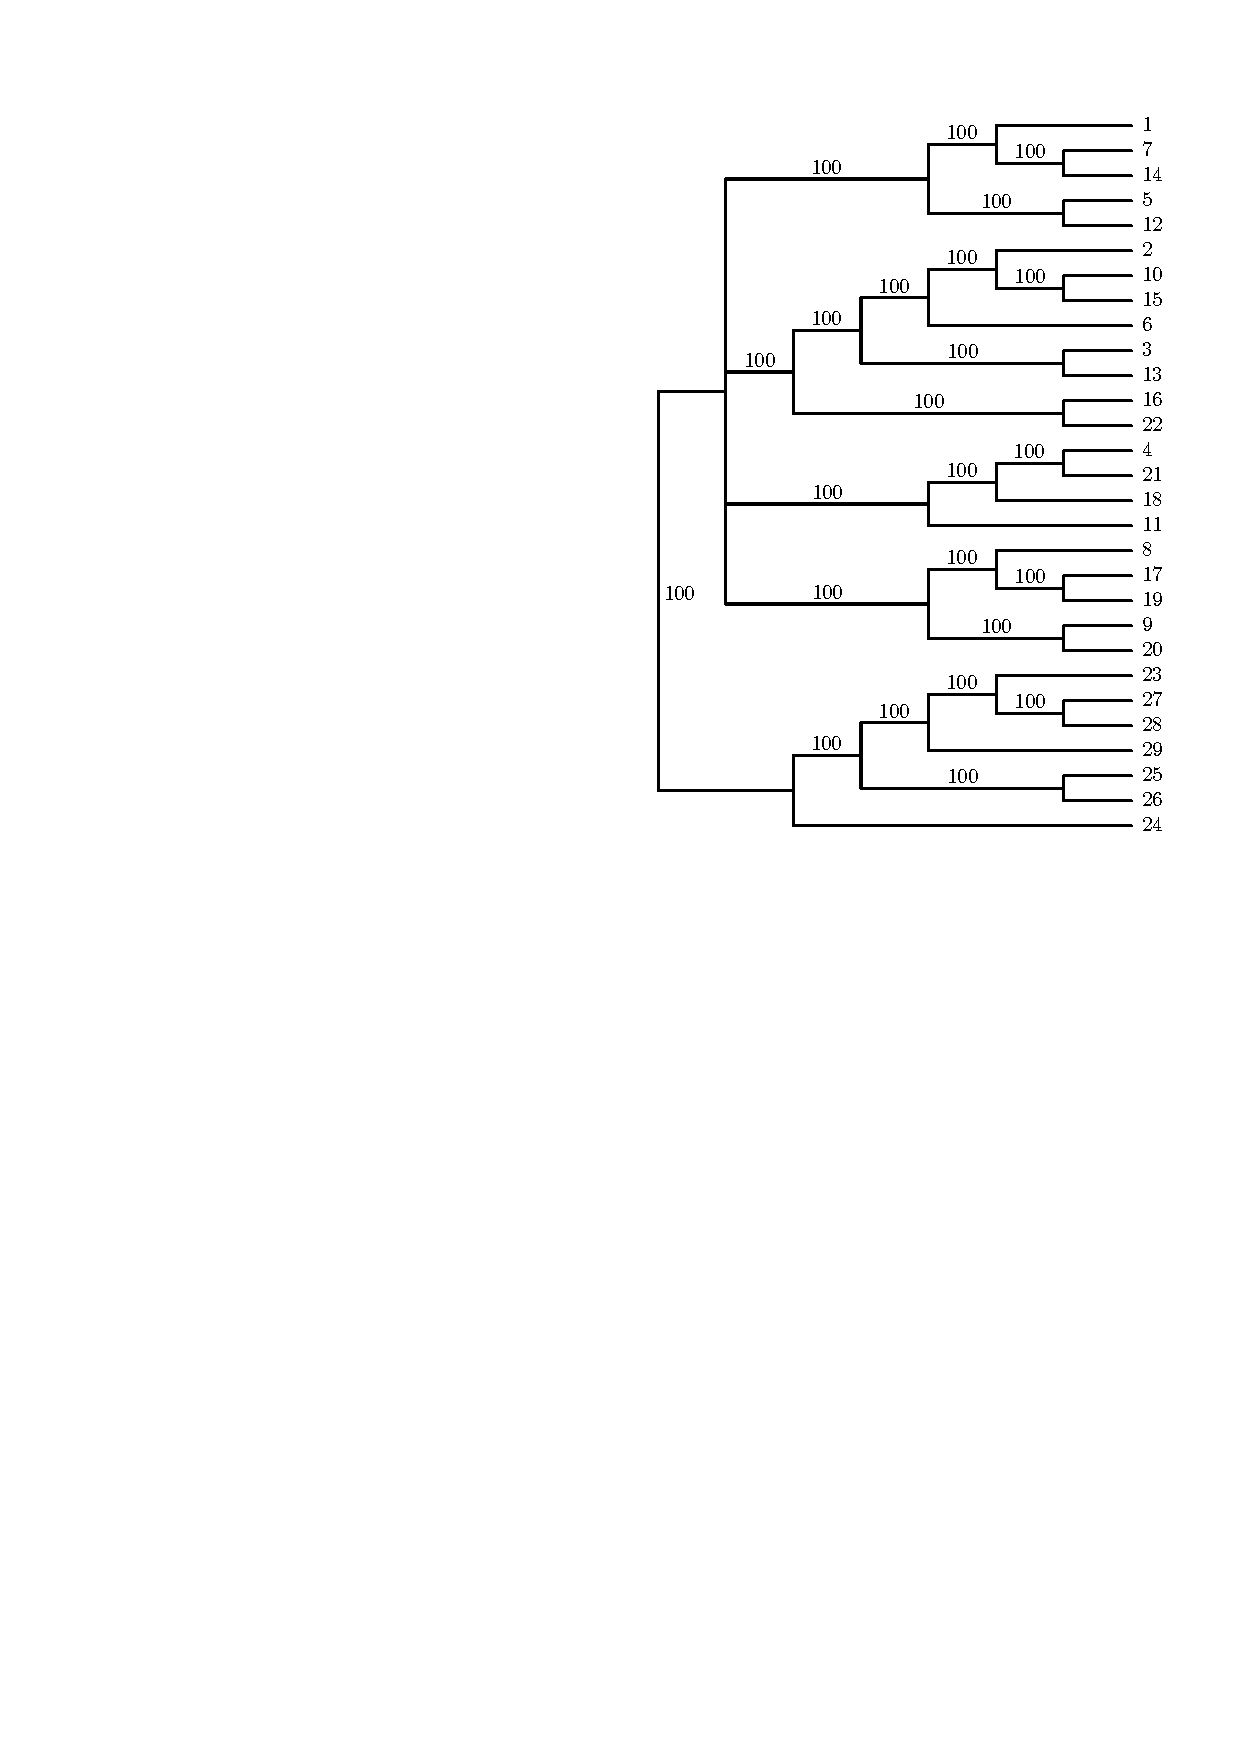
\includegraphics[width=0.5\textwidth]{mp-consensus.pdf}
                \caption{Majority rule consensus of the twelve most parsimonious trees. Values on branches indicate percent support.}
            \end{figure}
            
            \begin{figure}
                \centering
                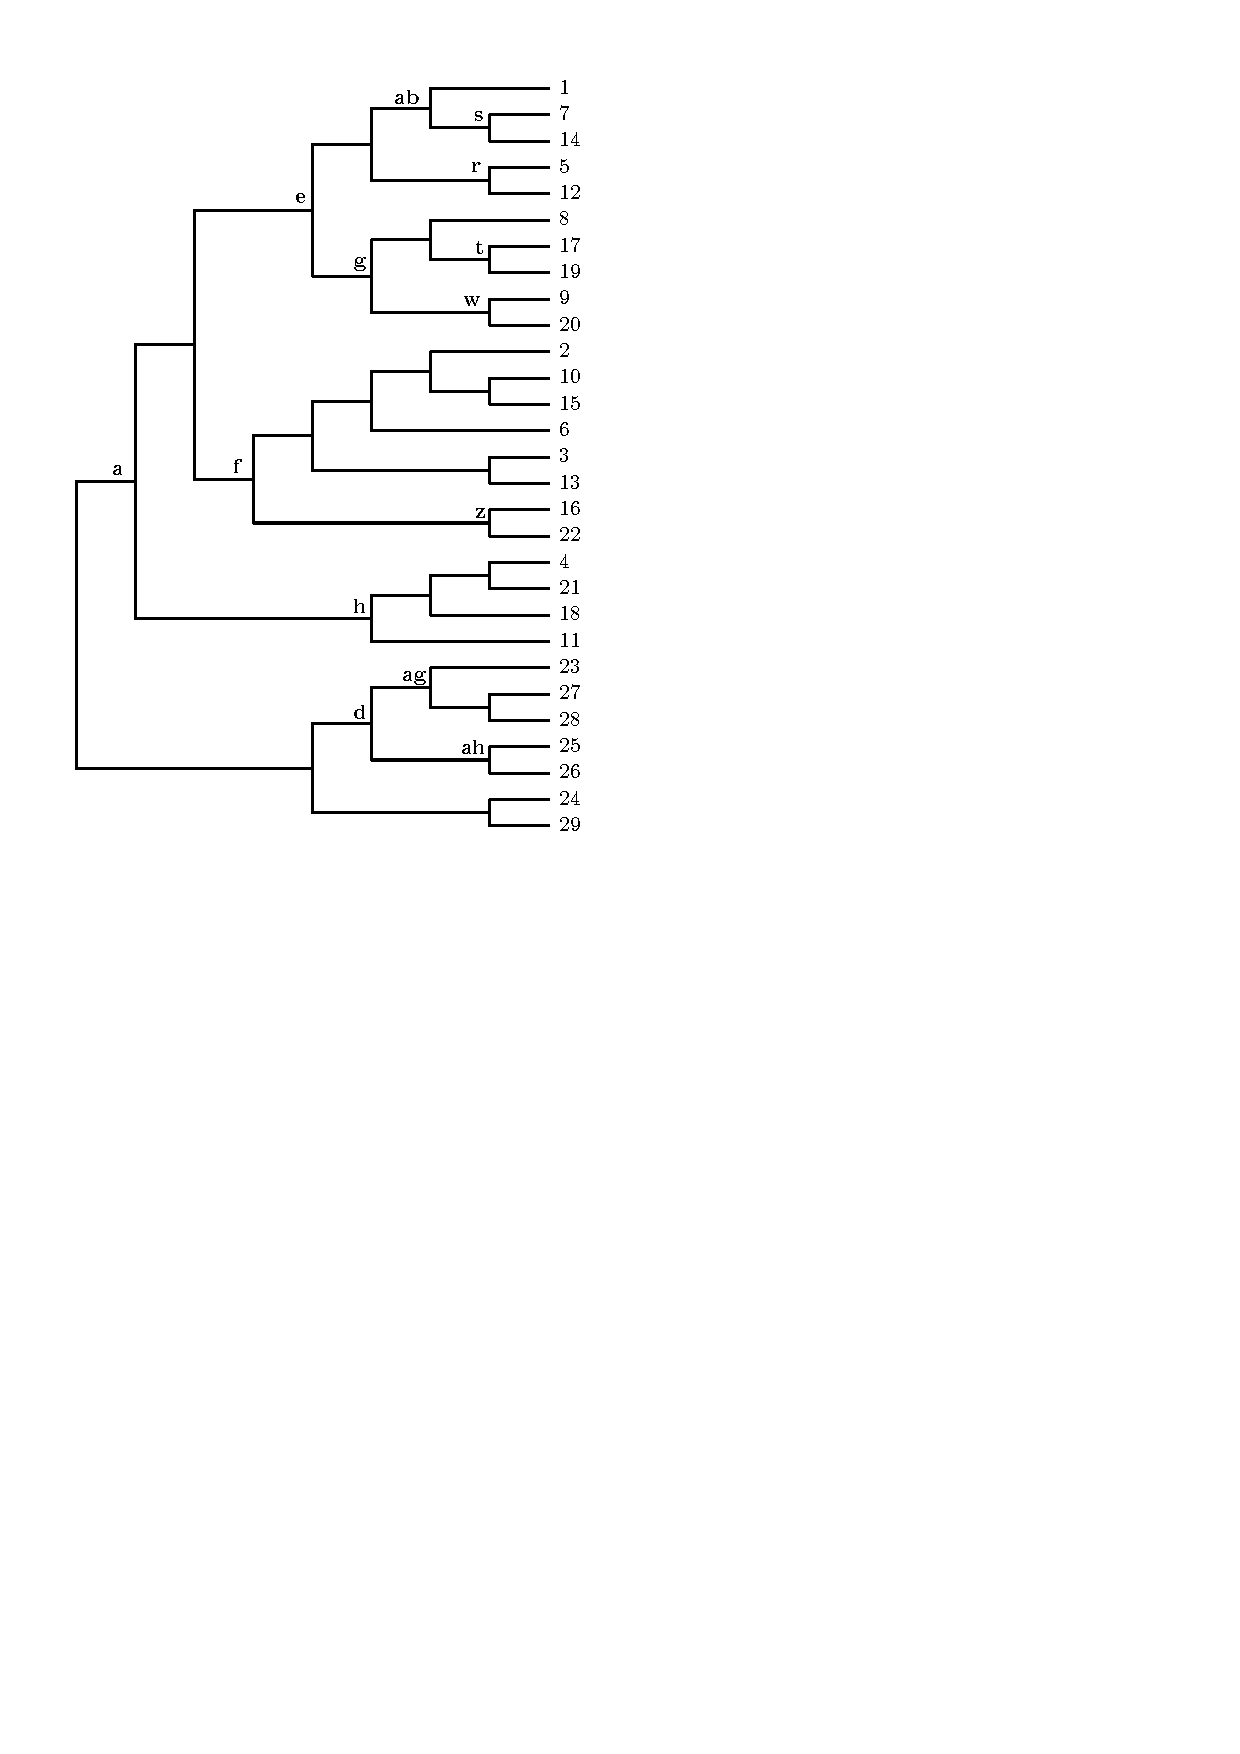
\includegraphics[width=0.5\textwidth]{mp.pdf}
                \caption{One of the twelve most parsimonious trees annotated with synapomorphies. Letters refer to the characters and table~1.}
            \end{figure}
            
            \begin{figure}
                \centering
                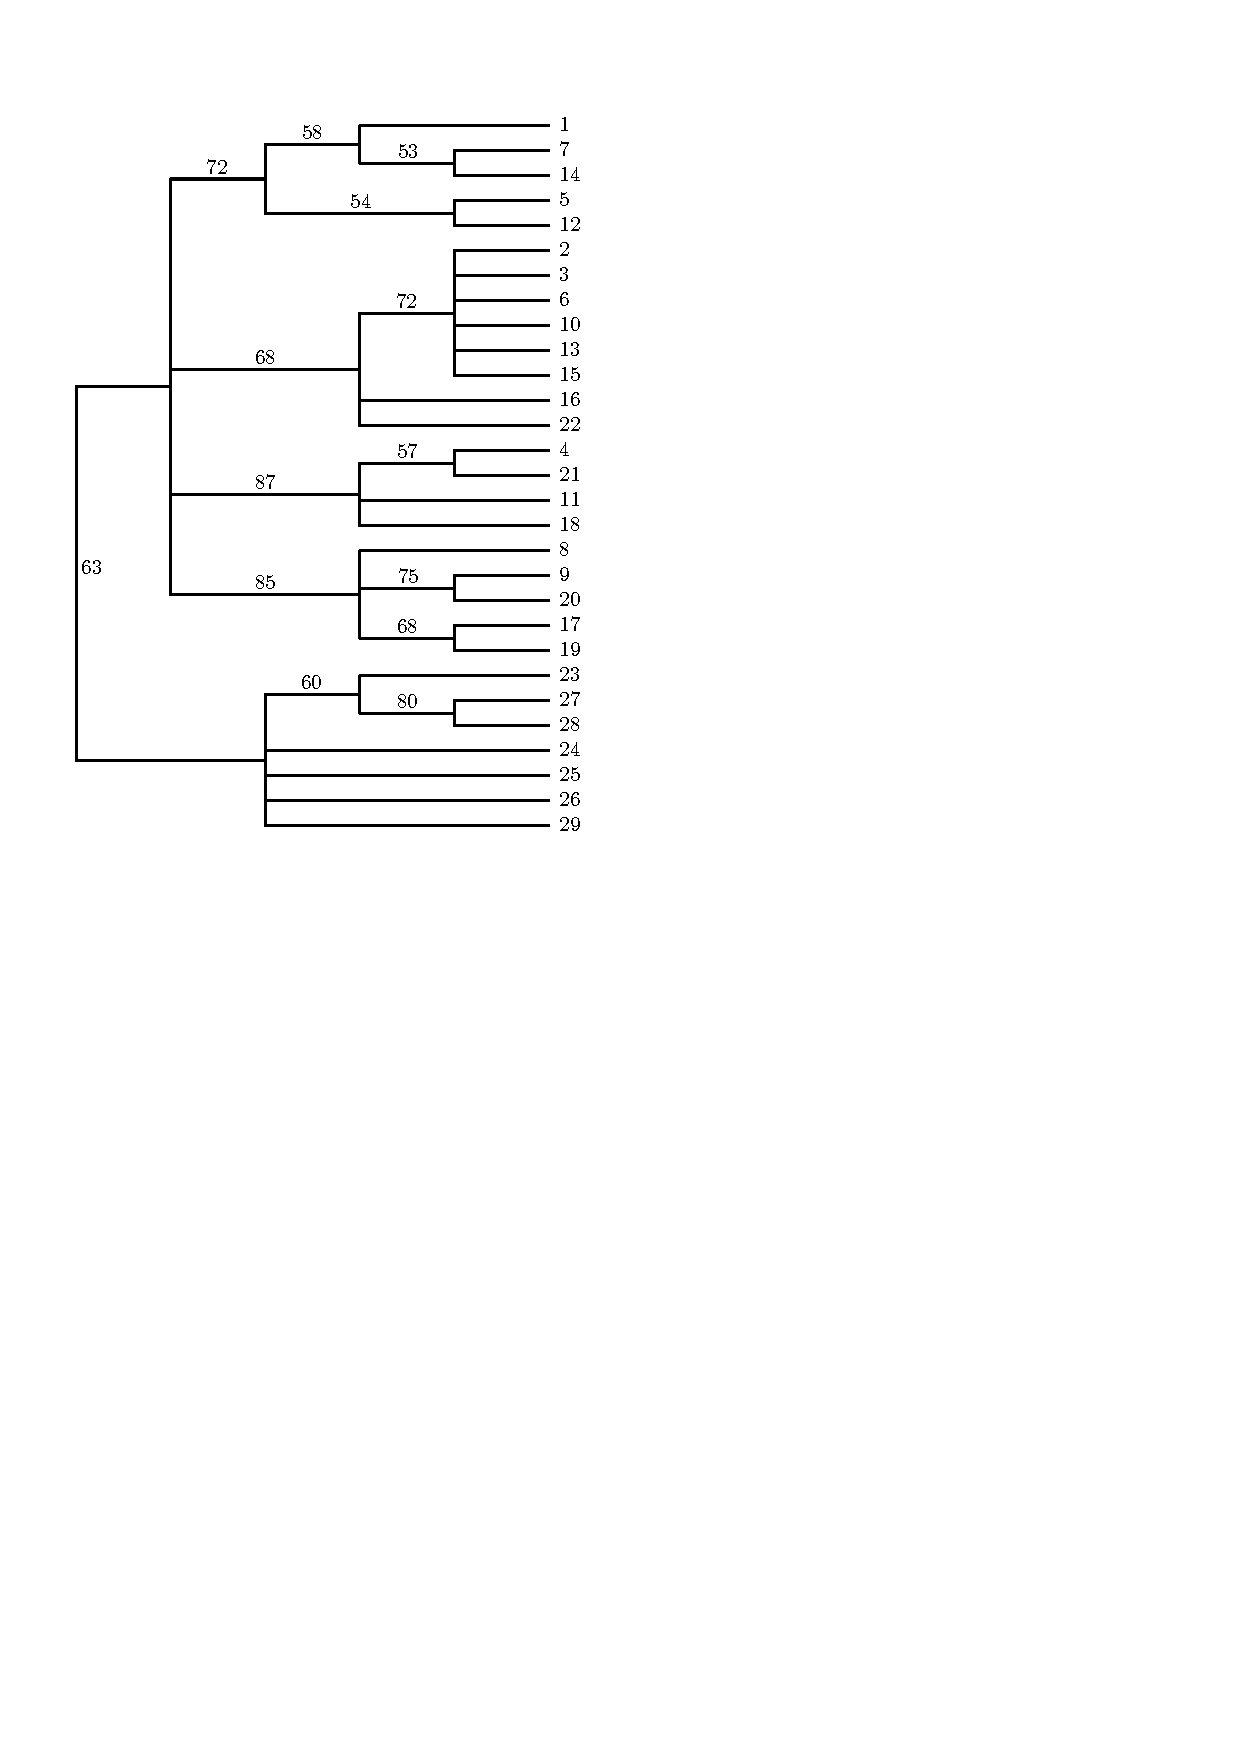
\includegraphics[width=0.5\textwidth]{bs.pdf}
                \caption{Majority rule consensus tree based on a bootstrap analysis with 1000 replicates. Values on branches indicate percent support.}
            \end{figure}
            

    \section*{Discussion}

            Overall, I was able to resolve the phylogeny of the Calminacules to a reasonable degree of precision.
            I summarised each species based on a set of traits and identified the major clades of the species and suggested a number of synapomorphies.

            A significant challenge was selecting characters such that the
                maximum parsimony reconstruction was fully bifurcating.
            I frequently returned to my data matrix to add additional characters or \enquote{fine-tune} existing characters to facillitate recovery of a bifurcating tree.
            Even with each tree fully bifurcating, the relationship between the major clades remained ambiguous between multiple maximum parsimony trees.
            This result suggests the presence of contradictory characters in the dataset or a lack of signal.
            
            The choice of characters obviously has a large impact on the analysis. The majority rule consensus tree from the bootstrapping operation clearly shows weak support for most of the clades. This suggests that the phylogeny is not very robust to changes in the choice of traits used to resolve the phylogeny. It may also be indicative of the presence of potentially contradictory states in the data matrix.
            The choice of outgroup may also have affected the analysis.
            Although using different outgroup (in place of clade B) is unlikely
                to change the phylogeny substantially, the character states of
                individuals in the new outgroup may affect our understanding of
                the ancestral traits in the phylogeny and therefore the
                synapomorphies, etc.
            
            An example of a synapomorphy from the dataset is the presence of eyes, which is a trait that is derived and shared by all of clade A. The respective synapomorphy is the lack of eyes, known based on the outgroup. It is important to note that there were no autapomorphies used to reconstruct the phylogeny, because they render no phylogenetic signal.
            
            Ultimately, the results of this effort are indicative that reconstructing a phylogeny from purely morphological characters is very challenging.
            Some of these challenges include identifying useful phenotypic traits objectively, dividing these traits into a reasonable number of discrete states, and gather enough signal from the data.
            Of course much of these issues are no longer present when using molecular data for phylogenetic analysis; however, a number of additional complexities such as molecular clocks, gene trees versus species trees, etc., emerge.

    \printbibliography

\end{document}
